\documentclass[10pt,a4paper]{article}
% WSPR Logger user guide. Built with:  pdflatex user_guide.tex  (twice; three times for the contents)
% The screenshots are in guide_img/ (taken from the running page with the station's own databases).
\usepackage[T1]{fontenc}
\usepackage[utf8]{inputenc}
\usepackage{mathptmx}
\usepackage[scaled=.92]{helvet}
\usepackage{courier}
\usepackage{microtype}
\usepackage[a4paper,margin=2.0cm,top=2.3cm,bottom=2.2cm,headsep=0.5cm]{geometry}
\usepackage{graphicx}
\usepackage{xcolor}
\usepackage{booktabs}
\usepackage{tabularx}
\usepackage{array}
\usepackage{enumitem}
\usepackage{caption}
\usepackage{float}
\usepackage{fancyhdr}
\usepackage{textcomp}
\usepackage{amsmath}
\usepackage{amssymb}
\usepackage{tikz}
\usetikzlibrary{arrows.meta,positioning}
\usepackage[hidelinks]{hyperref}

\definecolor{accent}{HTML}{0369A1}
\definecolor{boxbg}{HTML}{F1F6FA}
\definecolor{warnbg}{HTML}{FFF7E8}
\definecolor{warn}{HTML}{B45309}
\captionsetup{font=small,labelfont=bf,labelsep=period,justification=justified,singlelinecheck=false}
\setlist{itemsep=1.5pt,topsep=3pt,parsep=0pt}
\setlength{\parindent}{0pt}
\setlength{\parskip}{4.5pt plus 1pt}
\renewcommand{\arraystretch}{1.15}
\setcounter{tocdepth}{2}
\pagestyle{fancy}
\fancyhf{}
\fancyhead[L]{\small\itshape WSPR Logger --- how to read and use the web page}
\fancyhead[R]{\small\itshape User guide, version 1.2 --- November 2026}
\fancyfoot[C]{\small\thepage}
\renewcommand{\headrulewidth}{0.3pt}
\hypersetup{pdftitle={WSPR Logger - User guide},pdfauthor={Otso Laakso, OH2GAX}}

\newcommand{\km}{\,km}
\newcommand{\dB}{\,dB}
\newcommand{\MHz}{\,MHz}
\newcommand{\ui}[1]{\textsf{\small #1}}            % a word on the screen: button, switch, card title
\newcommand{\lead}[1]{\textbf{#1}\enspace}           % run-in paragraph head
\newcommand{\fig}[3]{\begin{figure}[H]\centering\includegraphics[width=#2\textwidth]{guide_img/#1}\caption{#3}\end{figure}}
\newcommand{\figpair}[5]{\begin{figure}[H]\centering
  \begin{minipage}[t]{0.485\textwidth}\centering\includegraphics[width=\textwidth]{guide_img/#1}\end{minipage}\hfill
  \begin{minipage}[t]{0.485\textwidth}\centering\includegraphics[width=\textwidth]{guide_img/#2}\end{minipage}
  \caption{#5}\label{#3}\end{figure}}
\newcommand{\infobox}[2]{\par\smallskip\noindent\fcolorbox{accent!60}{boxbg}{\begin{minipage}{\dimexpr\textwidth-2\fboxsep-2\fboxrule\relax}\small
  \textbf{#1}\enspace #2\end{minipage}}\par\smallskip}
\newcommand{\warnbox}[2]{\par\smallskip\noindent\fcolorbox{warn!60}{warnbg}{\begin{minipage}{\dimexpr\textwidth-2\fboxsep-2\fboxrule\relax}\small
  \textbf{#1}\enspace #2\end{minipage}}\par\smallskip}
% "How to read" block of an Analysis card
\newenvironment{reading}{\par\begin{description}[leftmargin=0pt,labelsep=0.4em,itemsep=2pt,font=\normalfont\bfseries]}{\end{description}\par}

\begin{document}
\thispagestyle{plain}
\begin{center}
{\small WSPR Logger project \quad$\cdot$\quad User guide, version 1.2 \quad$\cdot$\quad 9 November 2026}\par\vspace{10pt}
{\LARGE\bfseries WSPR Logger}\par\vspace{5pt}
{\large\bfseries How to read and use the web page:\\ the live map, history, statistics, propagation analysis and the car's track}\par\vspace{8pt}
{\normalsize Otso Laakso (OH2GAX)}\par
{\small home locator KP20jg, southern Finland \quad$\cdot$\quad \url{https://wspr.oh2gax.org} \quad$\cdot$\quad \url{https://github.com/oh2gax/wspr_logger}}
\end{center}
\vspace{2pt}

\infobox{In short.}{A small WSPR transmitter with GPS sends a 200\,mW signal on 20\,m from the roof of a car every ten minutes. Volunteer receivers all over the world decode it and upload what they heard to a public database. The WSPR Logger reads that database every ten minutes and shows, in one web page:
\begin{itemize}[leftmargin=1.2em]
\item \textbf{where the car is and how well it is heard now} --- the live map with the position, the stations that heard the last hour, the propagation estimate and the space weather (Section~\ref{sec:live});
\item \textbf{what happened at any earlier moment} --- the History Player replays every stored ten-minute snapshot on the live map (Section~\ref{sec:replay}), the History and Statistics pages show single days (Sections~\ref{sec:history}--\ref{sec:stats});
\item \textbf{what the history says about the band} --- the Propagation Analysis page: when the band opens, in which directions and how far the signal goes, how the ionosphere and the geomagnetic field change it, how the seasons compare, which days were unusual, and the chance of long-distance contacts in the coming hours (Section~\ref{sec:analysis}, the main part of this guide);
\item \textbf{where the car has been} --- the WPRS page turns the positions in the transmissions into a track (Section~\ref{sec:wprs}).
\end{itemize}
Section~\ref{sec:wspr} explains WSPR as far as needed to read the page; Section~\ref{sec:questions} lists questions you can answer with it, and Section~\ref{sec:limits} what the data cannot tell.}

\infobox{About the figures.}{All figures are screenshots of the page with the station's own data: the live map is shown as it was on 13 October 2026 at 12:14~UTC, the other pages with the data up to 6 November 2026. In the figures the map background is a plain outline of the continents; on the real page it is a detailed street map. The numbers on your screen will differ from the ones quoted here, because the data grows every ten minutes.}

{\small\tableofcontents}

\newpage
\section{WSPR in a nutshell}\label{sec:wspr}

\subsection{The signal and the network}
\lead{WSPR} (Weak Signal Propagation Reporter, pronounced ``whisper'') is a radio protocol designed to find out where a weak signal can be heard. A transmission lasts 110.6 seconds, starts one second after an even minute and occupies only about 6\,Hz in a 200\,Hz wide part of the band (on 20\,m: 14.0970--14.0972\,MHz). It carries the callsign, a Maidenhead locator and the transmit power. A receiver decodes it down to a signal-to-noise ratio of about $-30$\,dB, i.e.\ a signal a thousand times weaker than the noise in a normal 2.5\,kHz receiver bandwidth.

\lead{Receivers report what they hear.} Thousands of stations around the world listen on the WSPR frequencies around the clock, decode every transmission they can and upload the result to WSPRnet: who was heard, by whom, when, at what SNR and over which distance. The public mirror \texttt{wspr.live} makes all these reports available. A \emph{reporter} (or \emph{station}) on this page is one such receiving station.

\lead{The station.} The transmitter is a ZachTek WSPR transmitter of about 200\,mW (23\,dBm) with a built-in GPS receiver, feeding a Diamond monoband 14\,MHz whip on the roof of a VW Touran. It transmits once every ten minutes on 20\,m. Because the transmitter computes its six-character locator from the GPS fix, every report also says where the car was, to within about 4.6\,km.

\subsection{How the logger collects its data}
\begin{figure}[H]\centering
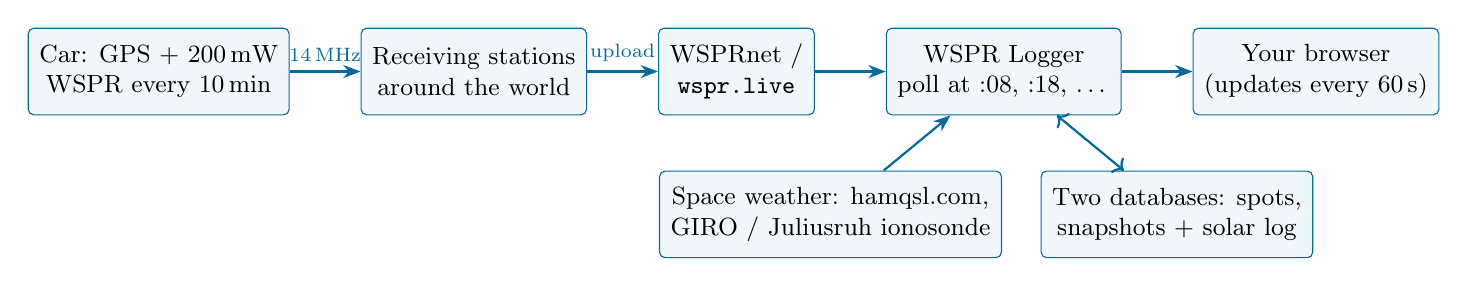
\begin{tikzpicture}[node distance=7mm and 9mm, every node/.style={font=\small}, box/.style={draw=accent, fill=boxbg, rounded corners=2pt, align=center, inner sep=4pt, minimum height=11mm},
  arr/.style={-{Stealth[length=2.2mm]}, accent, thick}]
\node[box] (tx) {Car: GPS + 200\,mW\\WSPR every 10\,min};
\node[box, right=of tx] (rx) {Receiving stations\\around the world};
\node[box, right=of rx] (db) {WSPRnet /\\\texttt{wspr.live}};
\node[box, right=of db] (lg) {WSPR Logger\\poll at :08, :18, \dots};
\node[box, right=of lg] (br) {Your browser\\(updates every 60\,s)};
\node[box, below=of lg, xshift=-22mm] (sw) {Space weather: hamqsl.com,\\GIRO / Juliusruh ionosonde};
\node[box, below=of lg, xshift=22mm] (dbs) {Two databases: spots,\\snapshots + solar log};
\draw[arr] (tx) -- node[above,font=\scriptsize]{14\,MHz} (rx);
\draw[arr] (rx) -- node[above,font=\scriptsize]{upload} (db);
\draw[arr] (db) -- (lg); \draw[arr] (lg) -- (br);
\draw[arr] (sw) -- (lg); \draw[arr, <->] (lg) -- (dbs);
\end{tikzpicture}
\caption{From the car to the page. The logger never talks to the receivers directly: it reads what they uploaded.}
\end{figure}

\lead{Every ten minutes.} Six minutes after each transmission slot (at minutes :08, :18, :28 \dots) the logger asks \texttt{wspr.live} for the reports of the last 45 minutes. Distant stations often upload a few minutes later than the nearby ones, so the last few slots are read again at every poll and their numbers are raised when late reports arrive (never lowered).

\lead{Two kinds of records.} The logger keeps
\begin{itemize}[leftmargin=1.2em]
\item a \textbf{spot} for each transmission that was heard: time, locator (the car's position), the number of stations that heard it and the farthest one. These feed the live map, the History and Statistics pages and the WPRS track;
\item a \textbf{snapshot} at every poll: the list of all stations that heard the beacon in the \emph{preceding 60 minutes}, each with its locator, best SNR and distance, together with the space weather of that moment. Snapshots feed the History Player and the Analysis page.
\end{itemize}

\lead{Space weather.} At every poll the logger also stores the solar flux (SFI), the K and A index, the X-ray class, the solar wind and the other indices from hamqsl.com, the maximum usable frequency MUF(3000) of the Juliusruh ionosonde in northern Germany (from the GIRO database) and its critical frequency foF2.

\lead{Three seasons.} The live logger started in May 2026. The two earlier summers (from July 2024) were rebuilt afterwards from \texttt{wspr.live}, which keeps every report. They contain the spots and the snapshots, but \textbf{no space-weather values}, because those were never recorded. That is why the space-weather charts of the Analysis page only cover 2026.

\infobox{Words used in this guide.}{\textbf{Transmission} or \textbf{spot}: one 2-minute WSPR transmission that somebody heard. \textbf{Station}, \textbf{reporter}: a receiving station (a callsign at a locator). \textbf{Snapshot}: what the logger stored at one poll --- the stations heard in the preceding 60 minutes. \textbf{Stations heard} on the Analysis page always means the number of stations in a snapshot. \textbf{DX}: a station farther than 6\,000\,km. \textbf{SNR}: signal-to-noise ratio in dB, as reported by the receiver (2.5\,kHz reference bandwidth). \textbf{UTC}: all times on the page are UTC (Finnish time is UTC\,+\,2, in summer UTC\,+\,3).}

\section{The page at a glance}\label{sec:page}
\begin{figure}[H]\centering
\begin{minipage}[c]{0.27\textwidth}\centering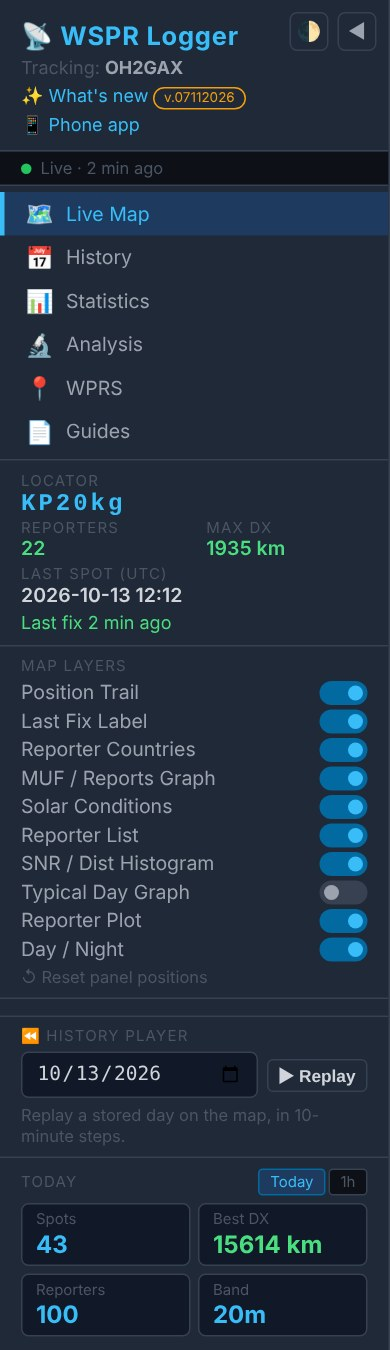
\includegraphics[width=\textwidth]{guide_img/live_sidebar.jpg}\end{minipage}\hfill
\begin{minipage}[c]{0.69\textwidth}\small
\lead{The menu (left pane).} From the top:
\begin{itemize}[leftmargin=1.1em]
\item the \textbf{title}, the tracked callsign and \ui{What's new} with the version label (a NEW marker until you open it);
\item the \textbf{theme button} (it cycles Auto, Dark and Light; Auto follows your computer) and \ui{$\blacktriangleleft$}, which hides the menu completely; the \ui{$\blacktriangleright$} handle on the left edge of the page brings it back;
\item the \textbf{status dot}: green when the newest spot is less than 20 minutes old, amber up to 2 hours, red beyond;
\item the \textbf{pages}: Live Map, History, Statistics, Analysis, WPRS and Guides;
\item the \textbf{Locator} block: the car's latest locator, the stations and farthest station of the latest transmission, and how old the latest fix is;
\item the \textbf{Map Layers} switches of the live map (Section~\ref{sec:live});
\item the \textbf{History Player} card: pick a day and press \ui{$\blacktriangleright$ Replay} (Section~\ref{sec:replay}); while it plays, the card shows the replayed moment with play / pause, the day steps and \ui{Live $\times$};
\item the \textbf{Today / 1h} cards: transmissions heard, best DX, most stations in one transmission and the band, for the UTC day or the last hour.
\end{itemize}
The History Player card and Today always stay at the bottom; on a short window the part above them scrolls. \ui{Phone app} under \ui{What's new} opens the phone view (see the \emph{Mobile app user guide}). The switches and their settings (MUF period and foF2, histogram tab, list order, Typical Day period, Today/1h, the place and size of panels you moved) are remembered in your browser; another browser or device keeps its own.
\end{minipage}
\caption{The menu on the left, with all Map Layers switched on.}
\end{figure}

\lead{What's new, User guides and About.} \ui{What's new} under the title and \ui{Guides} in the menu open one window with three tabs: short notes on each version, the PDF documents (this guide and the technical papers about the station), and a description of the station.

\lead{Links to a view.} The address in the browser follows what you look at: a History or Statistics day, the Analysis page, or a WPRS day and fix. Copy it and send it to someone, and the page opens on the same view (for example \texttt{\#wprs=2026-10-14\&days=5\&fix=120}).

\lead{Phones and small screens.} On a phone, use the phone view instead: \url{https://wspr.oh2gax.org/app} (\ui{Phone app} under \ui{What's new}), with one view at a time and every choice in a menu; it is described in the \emph{Mobile app user guide}. This page works on a small screen too: hide the menu with \ui{$\blacktriangleleft$} to give the map the whole screen; on the Analysis page the cards are stacked in one column.

\section{The live map}\label{sec:live}
\fig{live_overview.jpg}{1.0}{The live map on 13 October 2026 at 12:14 UTC with every layer switched on: the MUF graph across the top, Solar Conditions, the Reporter List and the SNR histogram on the left, the reporters as great-circle arcs on the map with the day/night terminator (dashed), and the Current Position, Propagation and Reporter Countries cards on the right.\label{fig:live}}

The live map opens by default and refreshes itself every minute; the data behind it changes every ten minutes, after each poll. The car is the round marker: \textbf{green} when the newest spot is less than an hour old, \textbf{red} when older. Beside it, the \ui{15 min ago} label (switch \ui{Last Fix Label}) says how old the position is: green up to 25 minutes (one transmission every ten minutes plus the upload delay), amber up to an hour, red beyond. The \ui{Position Trail} switch draws today's positions as a dashed line.

\begin{figure}[H]\centering
\begin{minipage}[c]{0.24\textwidth}\centering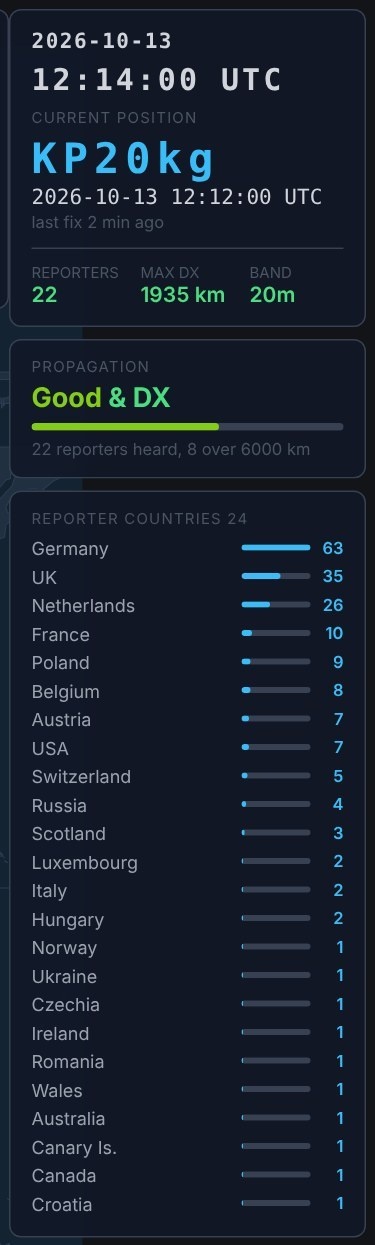
\includegraphics[width=\textwidth]{guide_img/live_cards.jpg}\end{minipage}\hfill
\begin{minipage}[c]{0.72\textwidth}\small
\lead{Current Position.} The UTC date and clock, the car's locator, the time of the latest heard transmission and its age, and for that transmission the number of stations that heard it, the farthest one (\ui{Max DX}) and the band. The values turn red when the spot is more than an hour old.

\lead{Propagation.} An estimate of the band from the stations that heard the latest transmission:

\begin{tabular}{@{}ll@{\hspace{14pt}}ll@{}}\toprule
Stations & Shown as & Stations & Shown as\\\midrule
up to 5 & Very low & 41--60 & Very good\\
6--10 & Low & 61--100 & Extremely good\\
11--20 & Normal & over 100 & Exceptional\\
21--40 & Good & & \\\bottomrule
\end{tabular}

\textbf{\& DX} is added when two or more of the stations of the last hour are beyond 6\,000\,km. \textbf{HIGH MUF} appears when the Juliusruh MUF is above 28\,MHz. \textbf{No propagation} means no spot for more than an hour; on 20\,m between 06 and 15~UTC, when silence is unusual, it says \textbf{No propagation or TX Fail} --- check the transmitter. \textbf{DB Timeout!} (amber) means \texttt{wspr.live} is not answering: the silence is the database's, not the band's.

\lead{Reporter Countries.} The countries of the stations of the last hour, with a bar and a count; a station with an unusual callsign is placed by its locator (for example \emph{W.\ Europe}).
\end{minipage}
\caption{The cards on the right of the live map.}
\end{figure}

\warnbox{Why does Current Position show fewer stations than the list?}{The card counts the stations that heard the \emph{latest transmission}, as far as they have uploaded by now; the Reporter List, the histogram, the plot and the countries cover \emph{all stations of the last 60 minutes}. In Figure~\ref{fig:live} the 12:12 transmission had 22 stations so far (more were still to come), while 193 stations heard the beacon in the last hour.}

\subsection{MUF / Reports graph}
\fig{live_muf.jpg}{1.0}{The MUF graph: Juliusruh MUF(3000) as the blue line, the stations of each transmission as green bars, for the last 2 days.}
The blue line is the \textbf{MUF(3000)} measured by the ionosonde at Juliusruh: the highest frequency that the ionosphere above Juliusruh would return to the ground over a 3\,000\,km path. Your 20\,m signal (14\,MHz) needs the MUF of its own path to be above 14\,MHz. The green bars are the stations that heard each transmission. Read the two together: in the morning the bars rise when the MUF climbs through about 14--16\,MHz, they stay high while the MUF is high, and they fall away in the evening when the MUF drops below about 12\,MHz. Use \ui{1d / 2d / 3d / 1wk} to change the span. The \ui{foF2} button adds a third line (amber) on the same MHz scale: the \textbf{foF2} of Juliusruh, the highest frequency the F2 layer returns straight up (Section~\ref{sec:iono}); the MUF over 3\,000\,km is about three times foF2. foF2 is stored from November 2026, when the Juliusruh monitor page became its source, so the line starts there. Juliusruh is about 1\,000\,km south-west of the car, roughly under the path to Central Europe, so it describes the busiest paths quite well and the paths to other directions only roughly.

\subsection{Solar Conditions}
\begin{figure}[H]\centering
\begin{minipage}[c]{0.36\textwidth}\centering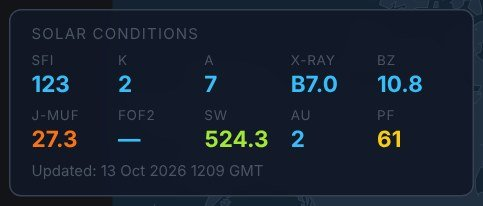
\includegraphics[width=\textwidth]{guide_img/live_solar.jpg}\end{minipage}\hfill
\begin{minipage}[c]{0.6\textwidth}\footnotesize
\begin{tabularx}{\textwidth}{@{}lX@{}}\toprule
Field & Meaning, and when it is coloured\\\midrule
SFI & solar flux at 10.7\,cm: the sun's activity (60--300) \\
K & geomagnetic disturbance, 0--9 (3-hour): green 0--1, orange 4--5, red 6+ \\
A & daily geomagnetic index: yellow-green 8--15 \dots\ purple 100+ \\
X-ray & solar flare class: C yellow, M orange, X red \\
Bz & north--south magnetic field of the solar wind (nT); south (negative) couples to the Earth's field: green to purple \\
J-MUF & Juliusruh MUF(3000) in MHz: grey below 8, green from 12, yellow 22+, red 30+ \\
foF2 & Juliusruh critical frequency (MHz), see Section~\ref{sec:iono} \\
SW & solar wind speed (km/s): coloured from 450 \\
AU & aurora activity 0--9: from 3 \\
PF & proton flux (pfu): from 50 (S1 radiation storm) \\\bottomrule
\end{tabularx}
\end{minipage}
\caption{Solar Conditions. A value is shown in the default colour when it is quiet; the colours rise with the disturbance (NOAA scales).}
\end{figure}
A MUF reading older than 3 hours is shown as \textbf{---}, because an old value must not look like the present one.

\subsection{Reporter List, SNR / Dist Histogram and Reporter Plot}
\begin{figure}[H]\centering
\begin{minipage}[c]{0.32\textwidth}\centering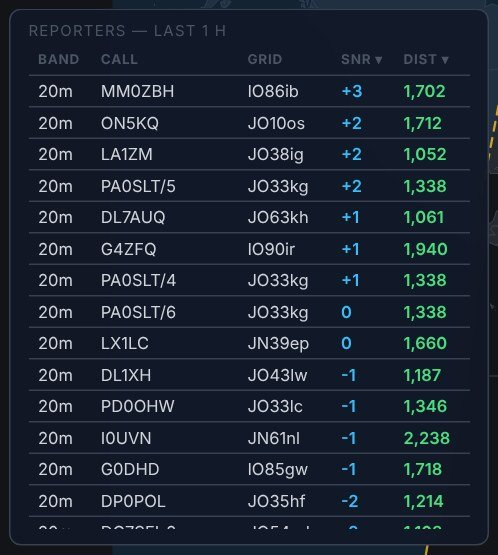
\includegraphics[width=\textwidth]{guide_img/live_reporters.jpg}\end{minipage}\hfill
\begin{minipage}[c]{0.32\textwidth}\centering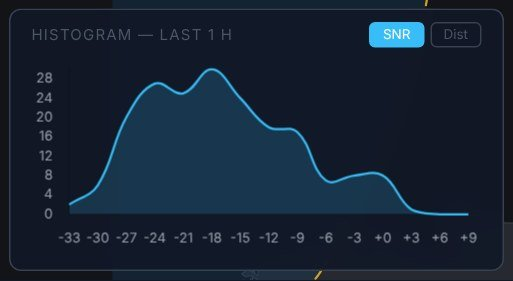
\includegraphics[width=\textwidth]{guide_img/live_hgram.jpg}\end{minipage}\hfill
\begin{minipage}[c]{0.32\textwidth}\small
\lead{Reporter List.} Every station of the last 60 minutes: band, callsign, locator, best SNR and distance. Click \ui{SNR} or \ui{Dist} to sort by it, largest first (\ui{$\blacktriangledown$}); click it again for the smallest first (\ui{$\blacktriangle$}) --- the weakest stations, or the nearest ones.

\lead{Histogram.} How these stations spread over SNR (3\,dB steps from $-33$ to $+9$\,dB) or, with \ui{Dist}, over distance. A peak far to the left means most stations hear you just above the decoding limit; a peak to the right, a strong signal.
\end{minipage}
\caption{Reporter List and SNR histogram of 13 October 2026 12:14: most stations hear the beacon at $-27$ to $-15$\,dB.}
\end{figure}

\fig{live_plot_europe.jpg}{0.9}{Reporter Plot over Europe: one circle per station, a great-circle line from the car to each; the stronger the signal, the thicker and brighter the line. Click a circle for callsign, locator, SNR and distance.}
\lead{Reporter Plot} draws each station of the last hour at its locator and a great-circle line from the car to it. The line weight and brightness follow the SNR, so the strongest paths stand out. Great-circle lines look curved on this map; they are the shortest paths on the globe (the line to Australia in Figure~\ref{fig:live} goes over Asia, as the signal does).

\lead{Day / Night} shades the night side of the Earth and draws the terminator (the grey line, dashed amber). Long-distance paths on 20\,m often open when one end is near the terminator (Section~\ref{sec:grey}).

\lead{Moving panels.} The Reporter List, the histogram, Solar Conditions, the Typical Day graph and Reporter Countries can be dragged by their titles anywhere on the map; the place is remembered. The Typical Day graph can also be resized from its lower right corner. Double-click a title, or \ui{Reset panel positions} in the menu, to put a panel back.

\subsection{Typical Day graph}
\fig{live_typ.jpg}{0.62}{The Typical Day graph on 6 November 2026 at 14:20 UTC, over 14 days: today (orange) a little below the usual in the morning and above it around noon.}
The \ui{Typical Day Graph} switch puts the \emph{Typical day (UTC)} card of the Analysis page (Section~\ref{sec:typday}) on the live map: for each UTC hour the median number of stations heard in 60 minutes over the period (blue line) and the range of the middle half of the days (shaded), with today in orange. So you see at a glance whether the band is doing better or worse than usual at this hour. \ui{7d / 14d / 30d / 90d} choose the period; 14 and 90 days are kept ready by the server, the others take a few seconds the first time. The graph is updated with the map; the panel opens at the bottom left, and can be moved and resized.

\section{The History Player}\label{sec:replay}
\fig{replay.jpg}{0.92}{The History Player on 13 October 2026 at 05:28 UTC: the terminator crosses Europe, only two stations (Italy, Russia) and a Greek station hear the car before the band opens. The bar at the bottom controls the replay.}
\fig{replay_bar.jpg}{0.8}{The player bar: play / pause, the time slider, the time and frame number, previous day, date, next day, speed and \ui{Live $\times$}.}
Pick a day in the \ui{History Player} card at the bottom of the menu and press \ui{$\blacktriangleright$ Replay} to replay it on the live map (a day without stored data opens the nearest earlier one), one frame for every ten-minute snapshot (including the polls when nobody heard the car, so the night is not skipped). The layers you have switched on show the replayed moment: the Reporter List, histogram and plot, Reporter Countries, Solar Conditions (with the MUF and foF2 of that moment), Day / Night (the terminator of that moment) and the Propagation card (from the spot logged at that time). The Current Position box follows the replay too: its date and time show the replayed moment in amber under \ui{REPLAY}, and below them the car's position at that moment, its stations and farthest station, and how old that fix was then; the car marker moves with it. A day without any logged position says so instead of showing the live position. Play at 1--16 frames per second, drag the slider, or step to the previous or next day that has data. \ui{Live $\times$}, in the bar or in the card, returns to the present. The $\blacktriangleright$ buttons on the Analysis page open the History Player at a chosen moment.

\infobox{Try this.}{Replay a summer day at 4 frames per second with Reporter Plot and Day / Night on: watch the band open in the morning as the terminator passes, the arcs spread over Europe at midday, and the long arcs to North America in the early morning or to Africa and Australia in the afternoon.}

\section{The History page}\label{sec:history}
\fig{history.jpg}{0.95}{The History page for 14 October 2026, the first day of a trip: the positions of the day on the map (green = first, blue = last) and every heard transmission in the table.}
Pick a date (or \ui{Today}, \ui{Yesterday}, \ui{$-$7 days}). The map shows the car's positions of the day as a track; the table lists every heard transmission with its time, locator, the number of stations and the farthest one. Click a marker for its details.

\section{The Statistics page}\label{sec:stats}
\fig{stats_top.jpg}{0.95}{Statistics for 13 October 2026: the day at a glance, \emph{Through the day} and \emph{Best DX per day} (the selected day highlighted in orange).}
\lead{The day at a glance.} Transmissions heard, the most stations in one transmission, the average, the longest DX (with its share of the all-time record, or a trophy on a record day), and the first and last heard transmission. $\blacktriangleleft$ and $\blacktriangleright$ step through the days.

\lead{Through the day.} Bars: the stations that heard each transmission; line: the farthest of them. A wall of bars from morning to evening is an open band; short spikes in the line are single long-distance reports.

\lead{Best DX per day.} One bar per day with the farthest station of the day; the line is the most stations in one transmission. Click a bar to open that day. 30\,d, 90\,d or All.

\lead{All-time records and Logged dates.} The best DX and the most stations ever, with the date each was set, the totals, and every date with data (click to open it).

\newpage
\section{The Propagation Analysis page}\label{sec:analysis}
The Analysis page turns the stored snapshots into answers about the band. Everything on it is computed from the logger's own databases; nothing is asked from \texttt{wspr.live}. The page opens at the last 14 days, which the server prepares in advance after every poll, so it appears at once. The other periods are computed when chosen and then kept for 10 minutes: the first opening of one can take some seconds (a message says so, and on a period change the old cards stay dimmed with \emph{Loading \dots} beside the buttons). The cards from \emph{Where you are heard} onwards load on their own after the rest.

\lead{The period.} The buttons at the top --- \ui{7 d}, \ui{14 d}, \ui{30 d}, \ui{90 d}, \ui{6 m}, \ui{1 yr}, \ui{All} --- choose the history that the cards use. When the last 14 days hold no reports (the transmitter is off, usually from November to March), the page opens at the first longer period that has some and says so beside the dates; a period chosen by hand is shown even when it is empty. Exceptions: the DX outlook always uses the whole history, \emph{Season against season} and \emph{Stations per month} cover all seasons, and the Ionosonde view has its own buttons. The figures of this section use \ui{All}: 4 July 2024 to 6 November 2026.

\infobox{Three ideas that the whole page uses.}{
\textbf{1. ``Stations heard'' is per snapshot.} It is the number of different stations that heard the beacon in the 60 minutes before a poll --- so it is smoother and larger than the stations of one transmission.

\textbf{2. The index: 100 = as usual at this hour.} The number of stations follows the time of day much more than anything else: about 3 in the small hours, about 75 at midday. Space weather follows the time of day too (the MUF is high in the daytime). Comparing raw averages would therefore mostly show the daily rhythm. Many cards use an \textbf{index} instead: the stations heard divided by what is typical for the same UTC hour (over the chosen period), times 100. \textbf{100} = as many stations as usual at that hour, \textbf{150} = half again as many, \textbf{50} = half. In the bar charts the bars at or above 100 are blue, the ones below orange, and a dashed line marks 100.

\textbf{3. DX share.} The green lines of many charts give the share of snapshots in which at least one station was beyond 6\,000\,km --- how often a long-distance path was open.}

\warnbox{What the charts can and cannot say.}{They describe this one station: one car, one antenna, 200\,mW, mostly from southern Finland. They show associations, not causes, and they cannot see a closed band and a switched-off transmitter apart. Small samples are noisy: a bar or a table row based on a few dozen snapshots can be far off. Most cards say how many snapshots stand behind a value --- hover a bar to see it.}

\subsection{The summary cards}
\fig{an_summary.jpg}{1.0}{The summary cards for the whole history.}
\begin{reading}
\item[Snapshots] how many polls the period holds, and over how many days (54\,868 over 495 days).
\item[Avg reporters] stations heard per snapshot, day and night together (56.3).
\item[Reporter $>$ 6000 km] share of snapshots with a DX station (16.3\,\%: a long-distance path is open about one hour in six).
\item[Farthest reporter] the longest distance in the period and when (15\,619\,km, Tasmania).
\item[Reporters $\sim$ MUF] two correlations between the stations heard and the Juliusruh MUF, from $-1$ to 1. \emph{Raw} compares the plain numbers (0.70 --- seemingly strong); \emph{vs.\ typical hour} first removes the daily rhythm (0.32). The second is the honest one: most of the raw correlation comes from both following the sun. A positive value still means more stations when the MUF is higher than usual for the hour.
\end{reading}

\subsection{Right now}
\fig{an_now.jpg}{1.0}{Right now: 116 stations at 14 UTC with a MUF of 26.9\,MHz --- typical when compared with similar MUF at this hour.}
\begin{reading}
\item[What it shows] the stations heard in the last 60 minutes next to what the history says for the same UTC hour: the median and the usual range (the middle half of the snapshots, 25--75\,\%), and the same for snapshots with a similar MUF (the same 2\,MHz step) when there are at least 8 of them.
\item[How to read it] \emph{Better than usual} = above the usual range, \emph{Below usual} = under it, \emph{Typical} = inside. The verdict uses the MUF comparison when it exists (it is the fairer one: a low count on a low-MUF day is not a surprise), otherwise the hour. In the figure the 116 stations are well above the hour's 78 but inside the 93--119 that is usual at a MUF of 26--28\,MHz.
\item[Watch out] no verdict is given while \texttt{wspr.live} is unreachable, and a MUF reading older than 3 hours is not used.
\end{reading}

\subsection{Ionosonde view}\label{sec:iono}
\fig{an_iono_day.jpg}{1.0}{Ionosonde view, \ui{Day}: 6 November 2026. Bars: stations heard per snapshot; orange: MUF(3000); green: foF2 (from 11:50 that day).}
\fig{an_iono_30.jpg}{1.0}{Ionosonde view, \ui{30 d}: each bar and point is an average over 3 hours. The daily MUF cycle and the stations heard rise and fall together; days with short or missing bars are days when the car was not transmitting or the band stayed poor.}
\begin{reading}
\item[What it shows] the stations heard (bars) with two values measured by the ionosonde at Juliusruh (lines). \textbf{foF2} is the \emph{critical frequency}: the highest frequency that the F2 layer reflects straight back up. \textbf{MUF(3000)} is the highest frequency that it returns over a 3\,000\,km hop; at an oblique angle the layer reflects about three times higher frequencies than straight up, so the MUF is roughly 3\,$\times$\,foF2.
\item[How to read it] for a 14\,MHz signal the MUF must be above 14\,MHz on the path. In the day view of 6 November the band opens at about 07~UTC as the MUF climbs through 15--20\,MHz, and the number of stations follows the MUF over the day. When the MUF stays below about 12\,MHz the bars stay short however active the sun is.
\item[Buttons] \ui{Day} shows every snapshot of one day ($\blacktriangleleft$ date $\blacktriangleright$); \ui{30 d} \dots\ \ui{All} and \ui{Custom} (a first and last day) show averages over 1 hour to 2 days, at most 500 bars, so that long periods stay readable; hover for the number of snapshots behind a bar. Polls that heard nobody count as 0 stations, so the night MUF is shown too.
\item[Watch out] MUF and foF2 exist only for the live-logged days from May 2026; foF2 is missing on many of them, because its first source (GIRO) often returned nothing --- the Juliusruh monitor page has been the source since November 2026. Juliusruh is about 1\,000\,km from the car: it describes the ionosphere near the middle of the busiest paths (to Central Europe) well, other directions less well.
\end{reading}

\subsection{Band-open heatmap}
\fig{an_heat.jpg}{1.0}{Band-open heatmap for the whole history: one column per day, one row per UTC hour (00 at the top). Yellow = most stations; dark = few; grey = no data.}
\begin{reading}
\item[What it shows] the whole period in one picture. Each cell is one UTC hour of one day, coloured by the average stations heard (or, with \ui{Farthest km}, the farthest station). The colour scale ends at the 97th percentile (given below the chart) so that a few extreme hours do not wash out the rest.
\item[How to read it] read it like a weather map of the band. The bright \emph{horizontal band} is the daytime opening; its upper and lower edges are the opening and closing times, and you can see them move with the seasons (a wider band around the equinoxes). \emph{Vertical dark stripes} are single bad days (a geomagnetic storm, the transmitter off). The wide grey blocks are the winters, when the car does not carry the antenna. Hover a cell for its value.
\item[In this station's data] three seasons; the autumn months are the brightest, midsummer the dullest (see also \emph{Season against season}).
\end{reading}

\subsection{DX outlook --- next 12 hours}
\fig{an_outlook.jpg}{1.0}{DX outlook at 14 UTC on 6 November 2026: a station beyond 6\,000\,km in Africa is \emph{possible} in the next 3 hours (22\,\%), most likely at 17 UTC (37\,\%).}
\begin{reading}
\item[What it shows] for each region that has produced DX reports, the chance (in percent) that at least one station of that region farther than 6\,000\,km hears the beacon in each of the next 12 UTC hours.
\item[How it is made] the starting point is history: on what share of days the region was heard in that hour. This is then adjusted for the present conditions --- whether the MUF is low, medium or high for the hour, and whether the K-index is quiet ($\le$\,2) or active ($\ge$\,3) --- assuming they persist. The adjustment is used only if it has proved itself: the model is fitted on the first 70\,\% of the days and tested on the rest, and the note below the table gives the result (the \emph{Brier score}: the mean squared error of the probabilities, smaller is better). In the figure the adjusted model scored 0.0513 against 0.0531 for the hour of the day alone --- 3.3\,\% better, a small gain, so it is applied.
\item[How to read it] darker green = more likely; \emph{likely} means at least 40\,\% in the next three hours, \emph{possible} 15--40\,\%, \emph{unlikely} below. Hover a cell for the plain hour-of-day value and the adjustment factors. It always uses the whole history.
\item[Watch out] it is a description of this station's history, not a physical forecast: a sudden storm or a flare is not foreseen.
\end{reading}

\subsection{Typical day}\label{sec:typday}
\fig{an_profile.jpg}{1.0}{Typical day: median stations heard per UTC hour (line) with the middle half of the snapshots (shaded), and the latest day in orange.}
\begin{reading}
\item[What it shows] for each UTC hour, the median stations heard over the period and the 25--75\,\% range (half of all snapshots of that hour lie inside the shaded bar); the orange line is the latest day.
\item[How to read it] the curve is the rhythm of the band. In this station's data it is near 3 between 00 and 04~UTC (closed), rises steeply between 05 and 08, stays at 70--80 from 08 to 18 and falls through 19--22~UTC. If the orange line runs above the shaded range, today is a good day; below it, a poor one. A narrow shaded bar means the hour is predictable; a tall one, that it varies a lot from day to day.
\end{reading}

\subsection{Reporters vs.\ MUF, K-index and solar flux}
\fig{an_muf.jpg}{0.62}{Reporters vs.\ Juliusruh MUF: index (bars, 100 = usual for the hour) and DX share (green) for each 2\,MHz step of MUF.}
\figpair{an_k.jpg}{an_sfi.jpg}{fig:ksfi}{}{Left: by K-index. Right: by solar flux (SFI) in steps of 10.}
\begin{reading}
\item[What they show] the snapshots are grouped by the space-weather value of their moment (MUF in 2\,MHz steps, K in whole numbers, SFI in steps of 10); for each group the bar is the \textbf{index} (100 = as many stations as usual at those hours) and the green line the \textbf{DX share}. Groups with fewer than 15 snapshots are left out; hover a bar for the count.
\item[MUF] the clearest relation on the page. With a MUF below about 16\,MHz the index is only 20--45: the band is barely open even at hours that are normally good. Between 18 and 20\,MHz it reaches 100, and from 20 to 28\,MHz it is 140--155, with a DX share around 20\,\%. Above 28\,MHz the groups are small and the bars jump about.
\item[K-index] a disturbed geomagnetic field weakens the F2 layer at high latitudes, which is where this station is. The index falls from 122 at K\,0 to about 90 at K\,3--4 and collapses at K\,6 (41) and K\,7 (8); the DX share falls from 22\,\% to almost nothing. A single high bar (here K\,5, 111) can come from a handful of days and should not be over-read.
\item[Solar flux] SFI describes the sun, not the ionosphere over the path, and changes slowly; on its own it explains little here. A higher SFI tends to raise the MUF over weeks, but within one season the MUF of the day matters far more.
\item[Watch out] these three charts use only the live-logged days of 2026; the rebuilt seasons have no space-weather values.
\end{reading}

\subsection{Geomagnetic storm days}
\fig{an_storms.jpg}{0.6}{Days when K reached 5 or more.}
\begin{reading}
\item[What it shows] every day of the period on which the K-index reached 5 (a minor storm) or more: the highest K and when it occurred, the average stations heard, the day's \textbf{index} against the typical day, and the snapshots behind it. $\blacktriangleright$ opens the moment of the K maximum in the History Player.
\item[How to read it] not every storm hurts: on 4 October 2026 the index was 120 although K reached 5, on 8 September only 62. Timing matters --- a storm that peaks at night or after the band has closed does less --- and so does its strength. Days with few snapshots (the car not used all day) are less reliable.
\end{reading}

\subsection{DX windows by hour and month by month}
\figpair{an_dxhour.jpg}{an_month.jpg}{fig:dxw}{}{Left: share of snapshots with a station beyond 6\,000\,km by UTC hour (bars) and the average farthest station (line). Right: month by month, average stations heard (bars) and DX share (line).}
\begin{reading}
\item[DX windows by hour] when the long-distance paths are open. This station has two windows: 03--07~UTC (up to 28\,\%: mostly North America, whose evening reaches the Finnish morning) and 09--12~UTC (26\,\%), with a minimum around 14~UTC (7\,\%) and a smaller evening rise (15\,\% at 17--18~UTC: Africa and Oceania). The line shows how far, on average, the farthest station of the hour is.
\item[Month by month] the seasons at a glance; hover for the days, snapshots and the average solar flux of the month. Compare the bars only between months with enough days --- a month with a few days of use is shown with the same width.
\end{reading}

\subsection{Grey line and long-distance windows}\label{sec:grey}
\fig{an_grey.jpg}{1.0}{The grey-line card: one chart per region (North America, Oceania, Africa, South America) with the sunrise ($\blacktriangle$) and sunset ($\blacktriangledown$) times at home (grey, H) and at the far end (colour, F).}
\begin{reading}
\item[What it shows] for each region: the share of days with a DX report from that region in each UTC hour (bars), with the times of sunrise and sunset at the home square and at the far end (the median position of the region's stations) as vertical lines, their spread over the period shaded.
\item[The test] long paths on 20\,m are known to favour the \emph{grey line}, the twilight zone where one end of the path is at sunrise or sunset. The card counts in how many of the region's DX hours the sun was within $\pm$6\textdegree\ of the horizon at either end, and compares this with the same UTC hours on the other days of the period (so the time of day is held fixed). \emph{Ratio} $>$\,1 means DX was more frequent when the terminator was on the path; \emph{z} says how sure: about 2 or more is a real difference.
\item[In this station's data] Africa: twilight in 40\,\% of its DX hours against 32\,\% expected (ratio 1.27, z\,=\,2.7) --- DX is somewhat more likely with the terminator on the path. North America and Oceania: ratio about 1.0 --- their windows are explained by the hour of the day alone.
\end{reading}

\subsection{Where you are heard and the distance distribution}
\figpair{amGeoCard.jpg}{amDistCard.jpg}{fig:geo}{}{Left: the stations by direction and distance from the home square. Right: the stations per 500\,km (logarithmic) and the share of reports.}
\begin{reading}
\item[Where you are heard] a compass rose seen from the home square, north up. Each ring is a distance band (to 1\,000, 2\,000, 3\,000, 6\,000, 10\,000\,km and beyond), each slice a direction of 22.5\textdegree. The colour of a cell is the number of stations there (or, with \ui{Reports}, how many reports they produced); a square-root scale keeps the quieter cells visible. Hover a cell for its numbers. The direction is the starting direction of the great-circle path from home --- the direction a beam antenna would point.
\item[How to read it] the bright cells are where the signal lands most often. Here 72\,\% of the stations are 1\,000--2\,000\,km away and 42\,\% lie to the west-south-west (the Netherlands, Belgium, the UK; most of Germany is in the next slice, south-west): the first hop of a 20\,m signal from southern Finland comes down in Western and Central Europe. The near ring is thin because the first hop skips over the nearest 1\,000\,km (the \emph{skip zone}). The outer rings show the long paths: North America to the north-west, Australia to the east.
\item[Distance distribution] the same stations as a histogram. The vertical axis is logarithmic (1, 10, 100, 1000), because otherwise the few distant stations would be invisible next to the thousands in Europe; the green line is the share of all reports in each step (90\,\% of the reports come from 1\,000--2\,000\,km). The dashed lines mark 6\,000 and 10\,000\,km. Here the median station is 1\,674\,km away; 156 stations are beyond 6\,000\,km and 32 beyond 10\,000\,km.
\end{reading}

\subsection{Band opening and closing}
\fig{amOpenCard.jpg}{1.0}{The first (green) and last (orange) transmission of each UTC day heard by 3 or more stations, with sunrise and sunset at home (grey dashed lines).}
\begin{reading}
\item[What it shows] for each day, the time of the first and of the last transmission that at least 3 stations heard --- when the band opened and closed for this signal --- next to sunrise and sunset at the home square.
\item[How to read it] the green dots follow sunrise and the orange dots follow sunset, both later. The band opens once the sun has built up the F2 layer: about half an hour after sunrise in October and November, two to three hours after it in April and May. It closes about three and a half hours after sunset in every month, while the layer slowly decays. In June and July the band often stays open all night (closing near midnight, opening again right after it) --- the sun at 60\textdegree\,N barely sets. Over the whole history the median opening is 05:22 and the median closing 20:52~UTC. Single dots far from the rest are days with a late start or an early stop of the transmitter, or a day with only a short opening.
\end{reading}

\subsection{Season against season and stations per month}
\figpair{amSeasonCard.jpg}{amMonthlyCard.jpg}{fig:season}{}{Left: median daytime stations per snapshot, by month and year. Right: stations per month and how many were new.}
\begin{reading}
\item[Season against season] the same calendar months of each year side by side: the median stations heard per snapshot in the daytime (08--17~UTC), or with \ui{DX > 6000 km} the share of snapshots with a DX station. A month is left empty when it has fewer than 50 daytime snapshots; hover for the days of data. Here October gives 61, 103 and 110 stations in 2024, 2025 and 2026, and the summers dip (in summer the daytime F2 layer at high latitudes is weaker than in spring and autumn). Differences between the years mix the sun's cycle, the number of active receivers and how much the car was used.
\item[Stations per month] blue: the different stations that heard the beacon in the month; green: those never heard before. The first month is all new; afterwards the green bars show how many newcomers each month brings (for example 172 of 765 in October 2026).
\end{reading}

\subsection{Signal strength by hour and by distance}
\figpair{amSnrHourCard.jpg}{amSnrDistCard.jpg}{fig:snr}{}{SNR of the reports: median (line) and middle half (shaded), by UTC hour (left) and by 1\,000\,km of distance (right).}
\begin{reading}
\item[What it shows] the SNR (dB in 2\,500\,Hz) that the stations reported: the median and the middle half of all reports, per UTC hour and per 1\,000\,km. Decoding stops near $-30$\,dB, so the lower edge is a floor.
\item[How to read it] by hour, the median stays near $-19$\,dB all day: when the band is open, the typical station hears the beacon about 10\,dB above the decoding limit. By distance, the SNR falls from $-17$\,dB at 0--1\,000\,km to about $-24$\,dB beyond 9\,000\,km --- the long paths are heard, but near the limit. Single bands can break the pattern (the last one here, $-14$\,dB at 15\,000\,km, is a few strong Australian stations).
\item[Watch out] only stations that \emph{decoded} the signal report an SNR. A poor hour therefore shows fewer reports, not lower SNRs; for how many stations hear you, use the other cards.
\end{reading}

\subsection{Unusual days}
\fig{amUnusualCard.jpg}{1.0}{The eight best and worst days of the period.}
\begin{reading}
\item[What it shows] the days whose daytime (06--18~UTC) differed most from what is typical for \emph{that month of the year} and those hours --- so a good October day is compared with other October days, not with midsummer. The \textbf{index} is 100 for a typical day; \emph{Avg} is the average stations heard per snapshot; the best days also give the farthest station, the worst days the highest K-index. Days with fewer than 36 daytime snapshots are not rated. $\blacktriangleright$ opens the day in the History Player (the best moment for a best day).
\item[How to read it] the best days are the openings worth replaying: 12 May 2026 had index 246, with up to 344 stations in one snapshot. The worst days point to storms (look at Max K) or to problems: a day with a quiet K and very few stations is often a transmitter or antenna problem.
\end{reading}

\subsection{Most loyal reporters}
\fig{amLoyalCard.jpg}{1.0}{The stations heard in the largest share of snapshots.}
The stations that hear the beacon most faithfully: the share of the period's snapshots they appear in, their distance, average and best SNR, and the day they were first heard in the period. Here G4ZFQ (England) appears in 72\,\% of all snapshots and ON5KQ (Belgium) in 69\,\%: these receivers listen around the clock and are about 1\,700--1\,900\,km away, in the busiest ring of the compass rose. Several entries with the same callsign and a suffix (/RE, /KE \dots) are usually separate receivers of one operator.

\subsection{Farthest reporters and excluded reports}
\fig{an_rec.jpg}{1.0}{The farthest stations of the period, one row per station, and the reports left out as implausible.}
The ten farthest stations of the period, one row per station with its longest distance; $\blacktriangleright$ opens that moment in the History Player. Below the table, \textbf{Excluded reports} lists the stations whose reported distance contradicts their own locator by more than 500\,km (for example SM4HVP: 17\,038\,km reported, 538\,km by its locator) --- a mistyped or stale locator. They are left out of every chart and record of the Analysis page. A reported distance of 0 means ``unknown'' and is not counted as a contradiction.

\newpage
\section{The WPRS page --- where the car has been}\label{sec:wprs}
\fig{wprs_days.jpg}{1.0}{The WPRS page with the trip of 14--18 October 2026: the days on the left, the visited squares (darker = more fixes), the track with a dot per fix, start (green), end (red), home (red ring) and the drive replay bar.}
\textbf{WPRS} (Whisper Position Reporting System) is the name of the idea of using WSPR as a position beacon. Each transmission carries the six-character locator that the transmitter computed from its GPS fix, so the heard transmissions form a track of the car with no mobile network or VHF coverage needed. The resolution is one Maidenhead subsquare, about 4.6\,$\times$\,4.6\,km here, and a fix exists only for a transmission that some station heard (at night, when the band is closed, there are gaps).

\lead{The day list.} One row per UTC day: squares and fixes, \emph{moved} (the largest distance between two squares used that day), the path length (summed distance between consecutive fixes) and, in amber, how far from home the car got. The \emph{home square} is the most frequent locator. The filter shows only days with at least the chosen movement or distance (any change of square, 5, 10, 25, 100, 150 or 200\,km; 10\,km is the default, because an ordinary trip between two neighbouring squares is 4.6--6.5\,km), and the span shows 1, 2, 3 or 5 days from the chosen one.

\begin{figure}[H]\centering
\begin{minipage}[c]{0.3\textwidth}\centering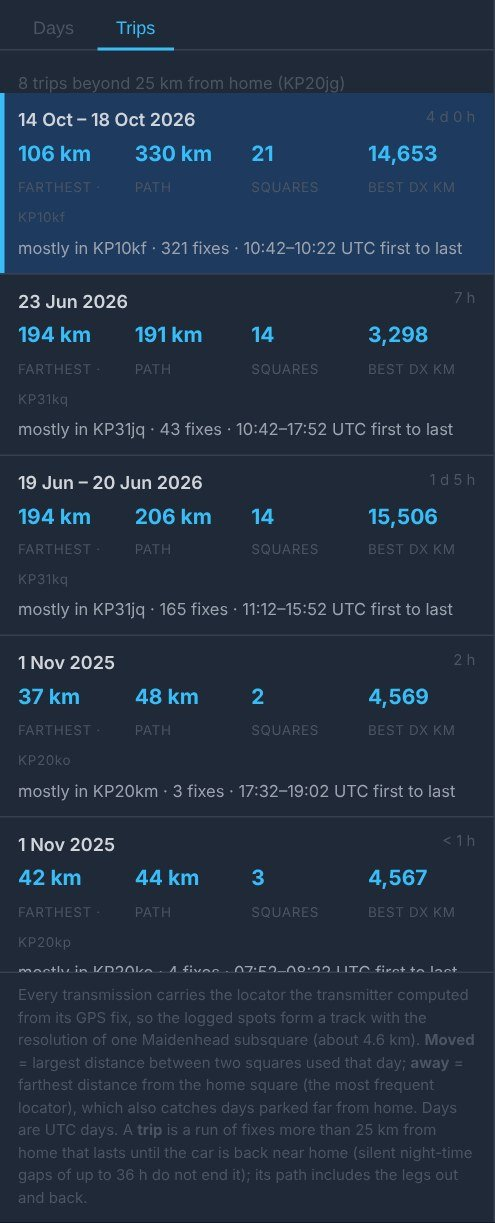
\includegraphics[width=\textwidth]{guide_img/wprs_trips.jpg}\end{minipage}\hfill
\begin{minipage}[c]{0.66\textwidth}\small
\lead{Trips.} The \ui{Trips} tab groups consecutive fixes more than 25\,km from home into trips; night-time silences of up to 36 hours do not end a trip. Each card gives the dates and duration, the farthest point and its square, the path, the number of squares, the best DX heard during the trip, the square used most and the first and last fix. Click a card to draw and replay the trip.

\lead{The map and the drive replay.} The squares visited are shaded by their number of fixes; the dashed line joins the fixes; hover a dot for its time, locator, stations and best DX. The \ui{DRIVE} bar plays the fixes in order (1--16 per second) and draws the trail so far in amber; the slider scrubs, $|\!\blacktriangleleft$ goes back to the start, and \ui{History Player} opens the shown moment on the live map, with the stations that heard the car there.

\lead{Copy link} gives an address that opens the same day, span and fix.
\end{minipage}
\caption{The trips of the whole history.}
\end{figure}

\warnbox{The track is public.}{Anyone can follow the car's position to within about five kilometres on the public WSPR databases while the transmitter is on.}

\section{What you can find out}\label{sec:questions}
\begin{table}[H]\centering\small
\begin{tabularx}{\textwidth}{@{}>{\raggedright\arraybackslash}p{4.6cm}>{\raggedright\arraybackslash}p{4.4cm}X@{}}\toprule
Question & Where to look & What to expect\\\midrule
Is the band open now, and how well? & Propagation card; Analysis \emph{Right now} & a level from Very low to Exceptional; \emph{Typical} or better against the hour and MUF \\
Is the transmitter working? & status dot, \emph{last fix} label, Propagation & a fix every 10 minutes in the daytime; \emph{No propagation or TX Fail} in the daytime is a warning \\
Which stations hear me, and how strongly? & Reporter List, histogram, Reporter Plot & most at $-27$ to $-12$\,dB, 1\,000--2\,000\,km to the south-west \\
Will a long-distance path open soon? & DX outlook; DX windows by hour & per region the chance in the next 12 hours; windows at 03--07 and 09--12~UTC \\
Why was today poor? & Ionosonde view, Solar Conditions, Storm days, Unusual days & a low MUF, a high K, or nothing --- then check the transmitter \\
When does the band open and close? & Band opening and closing; Typical day & 0.5--3\,h after sunrise; about 3.5\,h after sunset \\
How is this season compared with the last? & Season against season; Month by month & the same months side by side \\
Does the grey line help? & Grey line card; History Player with Day / Night & a ratio above 1 with z $\ge$ 2 \\
What was the best day, and what happened? & Unusual days $\blacktriangleright$, Farthest reporters $\blacktriangleright$ & opens the moment in the History Player \\
Where was the car on a day? & WPRS, History & track, squares and trips \\\bottomrule
\end{tabularx}
\caption{Questions and where to look.}
\end{table}

\section{Limitations}\label{sec:limits}
\begin{itemize}[leftmargin=1.2em]
\item \textbf{One station.} Everything describes one car, one antenna and 200\,mW, mostly from southern Finland. Another station, power or antenna would see a different band.
\item \textbf{Only what was heard and uploaded.} A transmission that nobody decoded leaves no trace; the logger cannot tell a closed band from a switched-off transmitter or a missing antenna. Late uploads are caught for 45 minutes.
\item \textbf{The receivers change.} The number of active receivers, especially in Europe, changes over the years and with the hours of the day; part of any difference between seasons comes from them, not from the band.
\item \textbf{Rebuilt seasons.} 2024 and 2025 were rebuilt from \texttt{wspr.live}; a check on a live-logged week found the same numbers (41.0 stations per snapshot both ways), but they have no space-weather values.
\item \textbf{One ionosonde.} The MUF and foF2 of Juliusruh describe the ionosphere about 1\,000\,km away, not on every path.
\item \textbf{Space weather is a feed.} The solar indices come from hamqsl.com and are only as fresh as their source; a K value is a three-hour value.
\item \textbf{Associations, not causes.} The charts show what happened together. The index method removes the daily rhythm but not, for example, the season.
\item \textbf{Small samples.} Groups with few snapshots are noisy; hover for the count. The Analysis page leaves out groups with fewer than 15 snapshots and days with fewer than 36 daytime snapshots.
\item \textbf{Implausible reports.} The Analysis page leaves out stations whose distance contradicts their locator (\emph{Excluded reports}). Everywhere else, a transmission whose farthest station was such a report shows its best distance as unknown (---), and it counts neither for the day's best nor for the all-time record. Until 7 November 2026 the all-time Best DX showed 17\,038\,km from SM4HVP, whose locator is only 538\,km away; the record is now 15\,619\,km.
\item \textbf{Position.} The WPRS track has the resolution of a subsquare (about 5\,km) and gaps when nobody hears the car.
\end{itemize}

\section{Quick reference}\label{sec:ref}
\begin{table}[H]\centering\small
\begin{tabularx}{\textwidth}{@{}>{\raggedright\arraybackslash}p{3.6cm}X@{}}\toprule
Item & Meaning\\\midrule
Spot, transmission & a 2-minute WSPR transmission that was heard: time, locator, stations, farthest station \\
Snapshot & the stations heard in the 60 minutes before a poll (every 10 minutes, at :08, :18 \dots) \\
Stations heard & the number of stations in a snapshot \\
DX & a station farther than 6\,000\,km; \emph{DX share}: share of snapshots with one \\
Index & stations heard compared with what is typical for the same UTC hour; 100 = typical \\
Usual range & the middle half (25--75\,\%) of the snapshots of the same hour \\
MUF(3000) & highest frequency returned over a 3\,000\,km hop (Juliusruh); 20\,m needs more than 14\,MHz \\
foF2 & the critical frequency of the F2 layer (straight up); MUF $\approx$ 3\,$\times$\,foF2 \\
K-index & geomagnetic disturbance 0--9; storm from 5 \\
SFI & 10.7\,cm solar flux, the sun's activity \\
SNR & signal-to-noise ratio in dB in 2\,500\,Hz; decoding limit about $-30$\,dB \\
Locator & Maidenhead: KP (field) 20 (square) jg (subsquare, about 4.6\,km) \\
Status dot & green $<$ 20\,min, amber $<$ 2\,h, red older \\
Fix age label & green $\le$ 25\,min, amber $\le$ 60\,min, red older \\
Grey line & the twilight zone; tested with the sun within $\pm$6\textdegree\ of the horizon \\
Brier score & mean squared error of a probability forecast; smaller is better \\
Links & \texttt{\#history=DATE}, \texttt{\#stats=DATE}, \texttt{\#analysis}, \texttt{\#wprs=DATE\&days=N\&fix=N} \\\bottomrule
\end{tabularx}
\caption{Terms and colours.}
\end{table}

\lead{More to read.} The \ui{Guides} tab also holds two papers written from this station's data: \emph{Twenty-metre WSPR propagation study} (three seasons in detail, with the methods behind the Analysis page) and \emph{WPRS --- Whisper Position Reporting System} (position beaconing with WSPR), with its two-page summary. The program and its documentation are at \url{https://github.com/oh2gax/wspr_logger}.

\vfill
{\small\textbf{Version history.}\quad 1.0, 7 November 2026: first version. \quad 1.1, 7 November 2026: the Analysis periods 7\,d and 14\,d and the opening at 14 days; implausible reports left out of the records too; country names from the locator; the History Player card in the menu and the replayed moment in the Current Position box; new screenshots of the live map, the History Player, Statistics and the info window. \quad 1.2, 9 November 2026: the Typical Day graph on the live map, foF2 in the MUF graph, the Reporter List sorted both ways, a shorter Locator block in the menu, the age label at the car shortened to \emph{N min ago}.}
\end{document}
